\chapter{Angles}\label{ChAngles}

\vspace{5cm}
\begin{acquis}
\begin{itemize}
\item Savoir repérer les angles formés par deux parallèles et une sécante (angles alternes-internes, angles alternes-externes, angles correspondants).
\item Savoir calculer des mesures d’angles en utilisant plusieurs propriétés (somme des angles d'un triangle, angles formés par deux parallèles et une sécante…).
\columnbreak
\item Savoir utiliser les propriétés des angles pour prouver que des droites sont parallèles ou perpendiculaires.
\item Savoir résoudre des problèmes en utilisant les angles.
\end{itemize}
\end{acquis}


\activites  
\begin{activite}[Les deux font la paire]



\begin{tabularx}{\linewidth}{XXXX}
\multicolumn{1}{c}{Figure 1} &
\multicolumn{1}{c}{Figure 2} &
\multicolumn{1}{c}{Figure 3} &
\multicolumn{1}{c}{Figure 4} \\
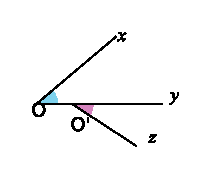
\includegraphics[width=.85\linewidth]{acti1} &
\includegraphics[width=.85\linewidth]{acti2} &
\includegraphics[width=.85\linewidth]{acti3} &
\includegraphics[width=.85\linewidth]{acti4} \\ 
\end{tabularx}

\begin{enumerate}
\item Dans les figures 2 et 4, les angles bleu et rose sont dits \textbf{adjacents}. Ce n'est pas le cas pour les autres figures. À partir de tes observations, essaie d'expliquer à quelles conditions deux angles sont adjacents. 
\item Deux angles adjacents ont-ils nécessairement la même mesure ? Justifie ta réponse.

\vspace{1em}

\begin{tabularx}{\linewidth}{XXXX}
\multicolumn{1}{c}{Figure 5} &
\multicolumn{1}{c}{Figure 6} &
\multicolumn{1}{c}{Figure 7} &
\multicolumn{1}{c}{Figure 8} \\
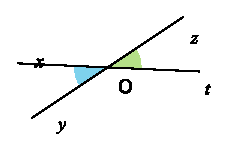
\includegraphics[width=.85\linewidth]{acti5} &
\includegraphics[width=.85\linewidth]{acti6} &
\includegraphics[width=.85\linewidth]{acti7} &
\includegraphics[width=.85\linewidth]{acti8} \\ 
\end{tabularx}

\item Dans les figures 5 et 8, les angles bleu et vert sont dits \textbf{opposés par le sommet}. Ce n'est pas le cas pour les autres figures. À partir de tes observations, essaie d'expliquer à quelles conditions deux angles sont opposés par le sommet.
\item Deux angles opposés par le sommet ont-ils nécessairement la même mesure ? Justifie ta réponse en utilisant une propriété sur deux angles symétriques par rapport à un point.
\end{enumerate}
\end{activite}


\begin{activite}[De jolies sommes !]
\begin{enumerate} \item Trace un triangle $ABC$ rectangle en $A$ puis mesure les angles $\widehat{ABC}$ et $\widehat{BCA}$.
\item Marie affirme que tous les élèves de la classe ne trouveront pas nécessairement les mêmes mesures mais qu'il y a quand même une relation entre ces deux mesures. Quelle est-elle ? Justifie ta réponse.

\vspace{1em}

On dit que deux angles sont \textbf{complémentaires} lorsque la somme de leurs mesures est égale à 90°. 
\item Les angles $\widehat{ABC}$ et $\widehat{BCA}$ sont-ils complémentaires ?
\item  Construis deux angles complémentaires \textbf{et} adjacents dont l'un mesure 64°.
\item Ahmed a mesuré l'angle $\widehat{xOz}$ ci-dessous et a trouvé 110°.

\begin{center}
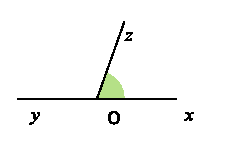
\includegraphics[width=.25\linewidth]{acti9}
\end{center}

Sa voisine lui dit que ce n'est pas possible et qu'à partir de l'erreur d'Ahmed elle pense connaître la bonne mesure. Quelle est cette mesure ? Comment a-t-elle pu la trouver ?

\vspace{1em}

On dit que deux angles sont \textbf{supplémentaires} lorsque la somme de leurs mesures est égale à 180°. 
\item Les angles $\widehat{xOz}$ et $\widehat{zOy}$ sont-ils supplémentaires ?
\item Construis deux angles supplémentaires \textbf{et} non adjacents dont l'un mesure 52°.
\end{enumerate}
\end{activite}


\begin{activite}[Avec des angles correspondants égaux...]
\begin{enumerate}
\item Observe la figure ci-dessous puis reproduis-la en choisissant la même mesure pour les angles $\widehat{ERF}$ et $\widehat{ESH}$.

\begin{center}
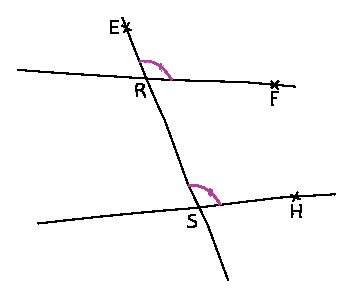
\includegraphics[width=.25\linewidth]{acti10}
\end{center}

\item\label{AactiquestionAngles} Comment peux-tu qualifier les angles $\widehat{ERF}$ et $\widehat{ESH}$ ? 
\item\label{AactiquestionDroites} Sur ta figure, quelle est la position relative des droites $(RF)$ et $(SH)$ ?
\item\label{AactiquestionPhrase} À l'aide des questions \ref{AactiquestionAngles} et \ref{AactiquestionDroites}, recopie puis complète la phrase : \textsl{« Si deux angles correspondants sont ... alors les deux droites coupées par la sécante sont ... . »}.
\item Écris une propriété identique à celle de la question \ref{AactiquestionPhrase} pour les angles alternes-internes.
\end{enumerate}
\end{activite}

\cours

\section{Caractériser deux angles ayant un sommet commun}

\begin{aconnaitre}
\textbf{Deux angles adjacents} sont deux angles qui ont un sommet commun, un côté commun et qui sont situés de part et d'autre de ce côté commun.

\vspace{.5em}

\textbf{Deux angles opposés par le sommet} sont deux angles qui ont un sommet commun et qui ont leurs côtés dans le prolongement l'un de l'autre.
\end{aconnaitre}

\begin{exemple*1}

Sur la figure ci-dessous, que peux-tu dire des angles $\widehat{AOB}$ et $\widehat{BOC}$ ?

\begin{center}
    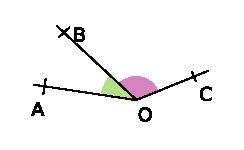
\includegraphics[width=.25\linewidth]{cours1}
\end{center}

\correction
Les angles $\widehat{AOB}$ et $\widehat{BOC}$ ont comme sommet commun le point $O$, comme côté commun la demi-droite $[OB)$ et sont placés de part et d'autre de $[OB)$ : ils sont donc adjacents.
\end{exemple*1}


\begin{exemple*1}
Sur la figure ci-dessous, que peux-tu dire des angles $\widehat{AOB}$ et $\widehat{DOE}$ ?

\begin{center}
    \includegraphics[width=.25\linewidth]{cours2}
\end{center}

\correction
Les angles $\widehat{AOB}$ et $\widehat{DOE}$ ont comme sommet commun le point $O$ et des côtés dans le prolongement l'un de l'autre ($A$, $O$, $D$ et $B$, $O$, $E$ sont alignés) : ils sont donc opposés par le sommet.
\end{exemple*1}

\vspace{1em}

Exercices « À toi de jouer »

Sur la figure ci-dessous, nomme trois paires d'angles adjacents.

\begin{center}
    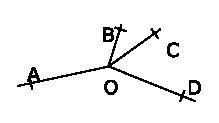
\includegraphics[width=.2\linewidth]{cours3}
\end{center}

Que dire des angles $\widehat{VST}$ et $\widehat{ESR}$ pour un parallélogramme $VERT$ de centre $S$ ?


\begin{aconnaitre}
Si deux angles sont opposés par le sommet \textbf{alors ils ont la même mesure.}
\end{aconnaitre}



\section{Angles complémentaires et supplémentaires}

\begin{aconnaitre}
\textbf{Deux angles complémentaires} sont deux angles dont la somme des mesures est égale à 90°.

\vspace{.5em}

\textbf{Deux angles supplémentaires} sont deux angles dont la somme des mesures est égale à 180°.
\end{aconnaitre}

\begin{exemple*1}
Sur la figure ci-dessous, que peux-tu dire des angles $\widehat{AOB}$ et $\widehat{BOC}$ ?

\begin{center}
    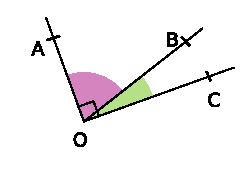
\includegraphics[width=.25\linewidth]{cours4}
\end{center}

\correction
Les angles $\widehat{AOB}$ et $\widehat{BOC}$ forment un angle droit : la somme des mesures de ces angles vaut 90°. Ce sont donc des angles complémentaires.
\end{exemple*1}

\begin{remarque}
Deux angles complémentaires et adjacents forment un angle droit. On peut donc en déduire que des droites sont perpendiculaires.
\end{remarque}


\begin{exemple*1}
Sur la figure ci-dessous, que peux-tu dire des angles $\widehat{AOB}$ et $\widehat{FED}$ ?

\begin{center}
    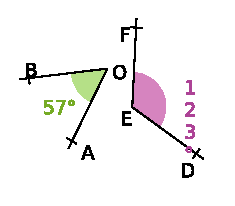
\includegraphics[width=.25\linewidth]{cours5}
\end{center}

\correction
$\widehat{AOB}+\widehat{FED}=57^\circ+123^\circ=180^\circ$ donc les angles $\widehat{AOB}$ et $\widehat{FED}$ sont supplémentaires.
\end{exemple*1}

\begin{remarque}
Deux angles supplémentaires et adjacents forment un angle plat. On peut donc en déduire que des points sont alignés.
\end{remarque}

\begin{remarque}
Deux angles complémentaires ou supplémentaires ne sont pas forcément adjacents.
\end{remarque}

\vspace{1em}

Exercices « À toi de jouer »

Les angles ci-dessous sont-ils complémentaires ?

\begin{center}
    
\includegraphics[width=.2\linewidth]{cours6}
\end{center}

Donne le complémentaire d'un angle de 27°.

Que peux-tu dire des angles aigus d'un triangle rectangle ? Justifie ta réponse.


Les angles ci-dessous sont-ils supplémentaires ?
\begin{center}
    
\includegraphics[width=.2\linewidth]{cours7}
\end{center}


Les points A, O et B sont-ils alignés ?
\begin{center}
    
\includegraphics[width=.2\linewidth]{cours8}
\end{center}







\section{Caractériser deux angles définis par deux droites et une sécante}


\begin{aconnaitre}
\begin{minipage}{.3\linewidth}
\centering
\includegraphics[width=.65\linewidth]{cours9}
\end{minipage}\hfill%
\begin{minipage}{.67\linewidth}
Les angles verts sont \textbf{alternes-internes}.

Ils sont déterminés par les droites $(d)$, $(d')$ et la sécante $(d_1)$.

Les angles roses sont \textbf{correspondants.}

Ils sont déterminés par les droites $(d)$, $(d')$ et la sécante $(d_2)$.
\end{minipage}
\end{aconnaitre}

\begin{exemple*1}
À l'aide de la figure, nomme des angles alternes-internes et des correspondants.

\begin{center}
    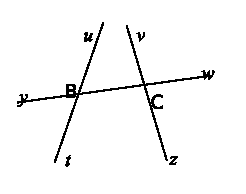
\includegraphics[width=.25\linewidth]{cours10}
\end{center}

\correction
Les droites $(ut)$, $(vz)$ et la sécante $(yw)$ forment :
\begin{itemize}
    \item deux paires d'angles alternes-internes qui sont : $\widehat{uBw}$ et $\widehat{yCz}$, $\widehat{vCy}$ et $\widehat{tBw}$.
    \item quatre paires d'angles correspondants qui sont : $\widehat{yBu}$ et $\widehat{vCy}$, $\widehat{yBt}$ et $\widehat{yCz}$, $\widehat{uBw}$ et $\widehat{vCw}$, $\widehat{tBw}$ et $\widehat{zCw}$.
\end{itemize}
\end{exemple*1}

\vspace{1em}

Exercices « À toi de jouer »

Sur la figure ci-dessous, les angles $\widehat{yOx'}$ et $\widehat{xEz'}$ sont-ils alternes-internes ? Justifie.

\begin{center}
    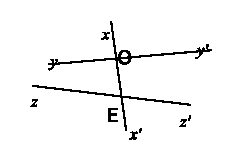
\includegraphics[width=.2\linewidth]{cours11}
\end{center}

Sur la figure  ci-dessous, nomme deux paires d'angles alternes-internes et quatre paires d'angles correspondants.

\begin{center}
    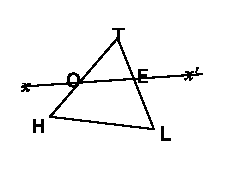
\includegraphics[width=.2\linewidth]{cours12}
\end{center}

\begin{aconnaitre}
Si deux angles alternes-internes sont déterminés par des droites parallèles \textbf{alors ils ont la même mesure.}

\vspace{.5em}

Si deux angles correspondants sont déterminés par des droites parallèles \textbf{alors ils ont la même mesure}.
\end{aconnaitre}

\begin{exemple*1}
Les droites $(vt)$ et $(uy)$ sont parallèles. Calcule la mesure des angles $\widehat{zEy}$ et $\widehat{vGw}$.

\begin{center}
    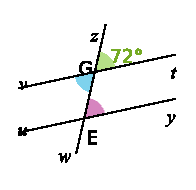
\includegraphics[width=.25\linewidth]{cours13}
\end{center}

\correction
Les angles correspondants $\widehat{zGt}$ et $\widehat{zEy}$ sont déterminés par les droites $(vt)$ et $(uy)$ qui sont parallèles. Ils sont donc de la même mesure. L'angle $\widehat{zEy}$ mesure donc 72°.

\vspace{.5em}

Les angles $\widehat{zGt}$ et $\widehat{vGw}$ sont opposés par le sommet. Ils sont donc de la même mesure. L'angle $\widehat{vGw}$ mesure donc 72°.
\end{exemple*1}

\vspace{1em}

Exercice « À toi de jouer »

Sur la figure ci-contre, les droites $(zz')$ et $(uu')$ sont parallèles. Calcule la mesure de l'angle $\widehat{x'Rz'}$ puis celle de l'angle $\widehat{uEx}$.

\begin{center}
    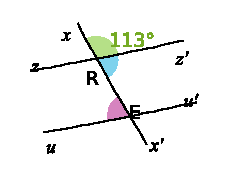
\includegraphics[width=.3\linewidth]{cours14}
\end{center}


\begin{aconnaitre}
Si deux angles alternes-internes sont de même mesure \textbf{alors les deux droites coupées par la sécante sont parallèles.}

\vspace{.5em}

Si deux angles correspondants sont de même mesure \textbf{alors les deux droites coupées par la sécante sont parallèles.}
\end{aconnaitre}


\begin{exemple*1}
Les droites $(yy')$ et $(zz')$ sont-elles parallèles ? Les droites $(xx')$ et $(uu')$ sont-elles parallèles ?

\begin{center}
    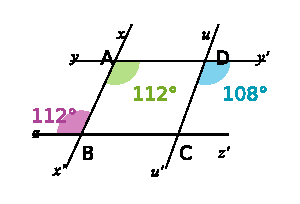
\includegraphics[width=.3\linewidth]{cours15}
\end{center}

\correction
Les angles $\widehat{x'Ay'}$ et $\widehat{xBz}$ déterminés par les droites $(yy')$, $(zz')$ et la sécante $(xx')$ sont alternes-internes. Les angles $\widehat{x'Ay'}$ et $\widehat{xBz}$ ont la même mesure.

Donc les droites $(yy')$ et $(zz')$ sont parallèles.

\vspace{.5em}

Les angles $\widehat{x'Ay'}$ et $\widehat{u'Dy'}$ déterminés par les droites $(xx')$, $(uu')$ et la sécante $(yy')$ sont correspondants. Si les droites $(xx')$ et $(uu')$ étaient parallèles alors les angles $\widehat{x'Ay'}$ et $\widehat{u'Dy'}$ seraient de la même mesure, ce qui n'est pas le cas.

Donc les droites $(xx')$ et $(uu')$ ne sont pas parallèles.
\end{exemple*1}

\vspace{1em}

Exercice « À toi de jouer »

Dans chacun des cas ci-dessous, indique si les droites $(AB)$ et $(OT)$ sont parallèles. Justifie ta réponse.

\begin{center}
\begin{minipage}{.48\linewidth}
\centering
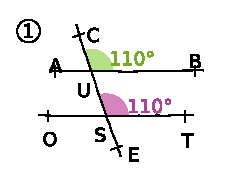
\includegraphics[width=.45\linewidth]{cours16}
\end{minipage}\hfill%
\begin{minipage}{.48\linewidth}
\centering
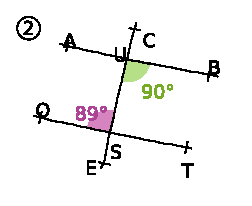
\includegraphics[width=.45\linewidth]{cours17}
\end{minipage}
\end{center}


\exercicesbase
\begin{colonne*exercice}
\serie{Propriétés des triangles}


\begin{exercice}[Reconnaître]
Donne, en justifiant, la nature de chacun des triangles s'il est particulier.
\begin{colenumerate}{4}
\item 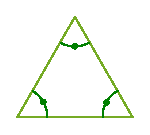
\includegraphics[width=.8\linewidth]{exoEnt1}
\item 
\includegraphics[width=.8\linewidth]{exoEnt2}
\item 
\includegraphics[width=.8\linewidth]{exoEnt3}
\item 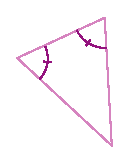
\includegraphics[width=.8\linewidth]{exoEnt4}
\end{colenumerate}
\end{exercice}



\begin{exercice}
Dans chaque cas, effectue un croquis puis construis la figure.
\begin{colenumerate}{1}
\item Trace un triangle $FIN$ rectangle en $F$ tel que $FI$ = 5 cm et $NF$ = 6 cm.
\item Trace un triangle $TRS$ rectangle en $S$ tel que $TS$ = 72 mm et $SR$ = 85 mm.
\item Construis un triangle $MNO$ équilatéral de côté 5 cm.
\item Construis un triangle isocèle $STU$ isocèle en $S$ tel que $ST$ = 58 mm et $TU$ = 32 mm.
\item Construis un triangle $ABC$ tel que $AB$ = 6 cm ; $BC$ = 5,2 cm et $CA$ = 42 mm.
\end{colenumerate}
\end{exercice}



\begin{exercice}[Médiatrices dans un triangle]
\begin{enumerate}
\item Construis un triangle $ABC$ tel que $AB$ = 5,7 cm, $AC$ = 5,3 cm et $BC$ = 7 cm.
\item Construis les médiatrices des segments $[AB]$ et $[CB]$. Note $O$ leur point d'intersection.
\item Construis la médiatrice du segment $[AC]$. Que constates‑tu ?
\item Trace le cercle de centre $O$ passant par $A$. Comment s'appelle ce cercle ?
\end{enumerate}
\end{exercice}



\begin{exercice}[Bissectrice dans un triangle]
\begin{enumerate}
\item Trace un triangle $UST$ tel que $UT$ = 6 cm ; $US$ = 10 cm et $ST$ = 14 cm.
\item Construis les bissectrices des angles $\widehat{UST}$, $\widehat{UTS}$ et $\widehat{TUS}$.

Que constates‑tu ?
\end{enumerate}
\end{exercice} 




\begin{exercice}
Dans les 6 cas suivants, détermine si la droite $d$ est :
\begin{enumerate}
\item une hauteur ;
\item une médiatrice ;
\item une bissectrice ;
\item une médiane.
\end{enumerate}

\begin{colenumerate}{3}
\item 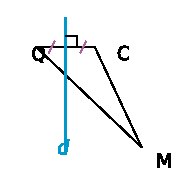
\includegraphics[width=.8\linewidth]{exoEnt5}
\item 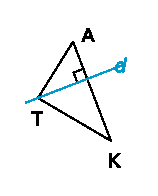
\includegraphics[width=.8\linewidth]{exoEnt6}
\item 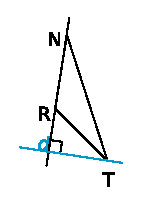
\includegraphics[width=.8\linewidth]{exoEnt7}
\item 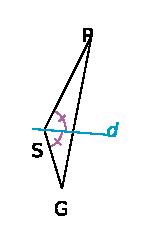
\includegraphics[width=.8\linewidth]{exoEnt8}
\item 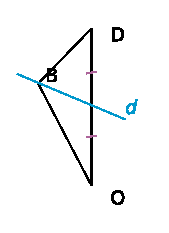
\includegraphics[width=.8\linewidth]{exoEnt9} 
\item 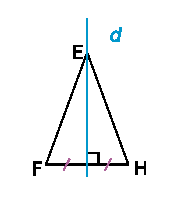
\includegraphics[width=.8\linewidth]{exoEnt10}
\end{colenumerate}
\end{exercice}




\begin{exercice}[Vocabulaire]
\begin{enumerate}
\item Construis un triangle $BOA$ tel que $BO$ = 5 cm, $OA$ = 7 cm et $AB$ = 8 cm. Trace la droite $d_1$ perpendiculaire à $[BO]$ et passant par $A$.
\item Trace la droite $d_2$ perpendiculaire au segment $[OA]$ et passant par son milieu.
\item Trace la droite $d_3$ qui coupe l'angle $\widehat{OBA}$ en deux angles égaux.
\item Trace la droite $d_4$ qui passe par $O$ et par le milieu de $[BA]$.
\item Détermine quelle(s) droite(s) représente(nt) la hauteur du triangle.
\item Détermine quelle(s) droite(s) représente(nt) une médiatrice.
\item Détermine quelle(s) droite(s) représente(nt) une bissectrice.
\item Détermine quelle(s) droite(s) représente(nt) une médiane.
\end{enumerate}
\end{exercice}




\begin{exercice}[Hauteurs d'un triangle]
Construis un triangle $BON$ tel que $BO$ = 68 mm, $BN$ = 62 mm et $NO$ = 45 mm.

Trace :
\begin{itemize}
\item en noir, la perpendiculaire à $(BN)$ passant par $O$ ;
\item en rouge, la perpendiculaire à $(NO)$ passant par $B$ ;
\item en vert, la perpendiculaire à $(BO)$ passant par $N$. Que remarques‑tu ?
\end{itemize}
\end{exercice}


\begin{exercice}[Hauteur (« relative à » ou « issue de »)]
\begin{enumerate}
\item Construis un triangle $AVE$ quelconque puis trace :
    \begin{itemize}
    \item en bleu, la hauteur issue du sommet $E$ ;
    \item en noir, la hauteur issue du sommet $A$ ;
    \item en rouge, la hauteur relative à $[AE]$.
    \end{itemize}
\item Observe ces trois hauteurs. Quelle remarque peux-tu faire ?
\end{enumerate}
\end{exercice}



\begin{exercice}[À l'intérieur ou pas ?]
\begin{enumerate}
\item Construis un triangle $DER$ ayant tous ses angles aigus. Trace les hauteurs de ce triangle.
\item Construis un triangle $NRV$ tel que $\widehat{NRV}$ soit un angle obtus. Trace les hauteurs de ce triangle.
\item Construis un triangle $GHT$ rectangle en $T$. Trace les hauteurs de ce triangle.
\item Observe les trois figures. Quelles remarques peux-tu faire ?
\end{enumerate}
\end{exercice}



\begin{exercice}[Vocabulaire] 
\begin{enumerate}
\item Construis un triangle $OA$. Trace la droite $(d_1)$ perpendiculaire à $[BO]$ et passant par $A$.
\item Trace la droite $(d_2)$ perpendiculaire au segment $[OA]$ et passant par son milieu.
\item Trace la droite $(d_3)$ qui coupe l'angle $\widehat{BOA}$ en deux angles égaux.
\item Trace la droite $(d_4)$ qui passe par $O$ et par le milieu de $[BA]$.
\item Reformule les questions précédentes en utilisant les mots : médiatrice, bissectrice, médiane et hauteur.
\end{enumerate}
\end{exercice}



\begin{exercice}[Cercles circonscrits]
Dans chaque cas, construis le triangle $LYS$ puis son cercle circonscrit.
\begin{enumerate}
\item $LS$ = 8 cm, $\widehat{YLS}$ = 65° et $\widehat{YSL}$ = 45°.
\item $LS$ = 4 cm, $LY$ = 5 cm et $\widehat{YLS}$ = 103°.
\item $LYS$ est isocèle en $L$ tel que $LY$ = 8 cm et $YS$ = 5,5 cm.
\item $LYS$ est un triangle équilatéral de côté 6 cm.
\end{enumerate}
\end{exercice}




\begin{exercice}[Sois malin !]
\begin{enumerate}
\item Construis un triangle $MEC$ tel que son cercle circonscrit ait un rayon de 5 cm.
\item Construis un triangle $RNB$ isocèle en $B$ avec $BN$ = 4 cm tel que son cercle circonscrit ait un rayon de 5 cm.
\end{enumerate}
\end{exercice}



\begin{exercice}[Cercle inscrit]
Dans chaque cas, construis le triangle $ABC$ puis son cercle inscrit.
\begin{enumerate}
\item $AC$ = 8 cm, $\widehat{BAC}$ = 60° et $\widehat{ACB}$ = 50°.
\item $AC$ = 10 cm, $AB$ = 8 cm et $\widehat{BAC}$ = 45°.
\item $ABC$ est isocèle en $A$ tel que $AB$ = 9 cm et $BC$ = 6 cm.
\item $ABC$ est un triangle équilatéral de côté 7,5 cm.
\end{enumerate}
\end{exercice}



\serie{Utiliser le vocabulaire associé aux angles}






\begin{exercice}
$\hat{a}$ et $\hat{b}$ sont deux angles complémentaires.

Calcule la mesure de $\hat{b}$ si :

$\hat{a}$ = 45°,\hfill%
$\hat{a}$ = 37°,\hfill%
$\hat{a}$ = 2°,\hfill%
$\hat{a}$ = 88,3°.  
\end{exercice}



\begin{exercice}
$\hat{x}$ et $\hat{y}$ sont deux angles supplémentaires.

Calcule la mesure de $\hat{y}$ si :

$\hat{x}$= 103°,\hfill%
$\hat{x}$= 95°,\hfill%
$\hat{x}$= 56°,\hfill%
$\hat{x}$= 0,3°.
\end{exercice}




\begin{exercice}
Indique si les angles proposés sont adjacents, complémentaires ou bien encore supplémentaires. Justifie tes réponses. 

\begin{center}
    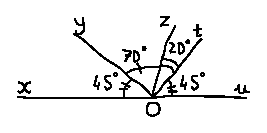
\includegraphics[width=.8\linewidth]{exoEnt11}
\end{center}

\begin{enumerate}
\item $\widehat{yOz}$ et $\widehat{zOt}$ ;
\item $\widehat{xOy}$ et $\widehat{yOu}$ ;
\item $\widehat{xOy}$ et $\widehat{tOu}$ ;
\item $\widehat{yOu}$ et $\widehat{tOu}$ ;
\item $\widehat{xOz}$ et $\widehat{zOt}$ ;
\item $\widehat{xOt}$ et $\widehat{uOt}$.
\end{enumerate}
\end{exercice}


\columnbreak
\begin{exercice}[Les deux font la paire]
Nomme, en justifiant, deux angles de la figure, codés ou non :
\begin{enumerate}
\item complémentaires et adjacents ;
\item complémentaires et non adjacents ;
\item supplémentaires et adjacents ;
\item supplémentaires et non adjacents ;
\item opposés par le sommet.
\end{enumerate}

\begin{center}
    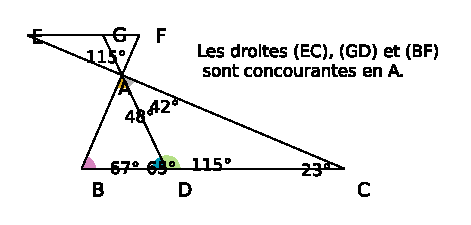
\includegraphics[width=\linewidth]{exoEnt12}
\end{center}

\end{exercice}




\begin{exercice}[Les angles inconnus]
\begin{enumerate}
\item Trouve la mesure de deux angles complémentaires, sachant que l'un d'eux est 8 fois plus grand que l'autre.
\item Trouve la mesure de deux angles supplémentaires, sachant que l'un d'eux est 9 fois plus petit que l'autre.
\end{enumerate}
\end{exercice}



\begin{exercice}[Des angles dynamiques...]
\begin{enumerate}
\item À l'aide du logiciel \emph{TracenPoche}, construis deux angles complémentaires et adjacents.
\item Propose une façon de procéder pour que ces angles restent adjacents, complémentaires et égaux à 45°, même quand on bouge les points.
\end{enumerate}
\end{exercice}



\begin{exercice}
Que peut-on dire des angles :

\begin{minipage}{.3\linewidth}
\begin{enumerate}
\item 1 et 3 ?
\item 1 et 5 ?
\item 3 et 5 ?
\item 1 et 4 ?
\item 4 et 6 ?
\item 3 et 7 ?
\end{enumerate}
\end{minipage}\hfill%
\begin{minipage}{.67\linewidth}
\centering
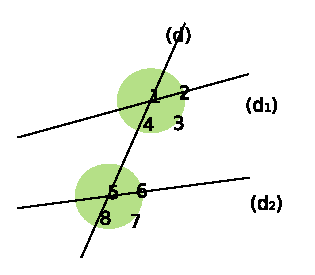
\includegraphics[width=\linewidth]{exoEnt13}
\end{minipage}
\end{exercice}




\begin{exercice}
Nomme deux angles de la figure et précise le nom de la sécante correspondante :
\begin{enumerate}
\item alternes-internes avec l'angle \no 3 ;
\item correspondants avec l'angle \no 10 ;
\item alternes-internes avec l'angle \no 13 ;
\item correspondants avec l'angle \no 7.
\end{enumerate}

\begin{center}
    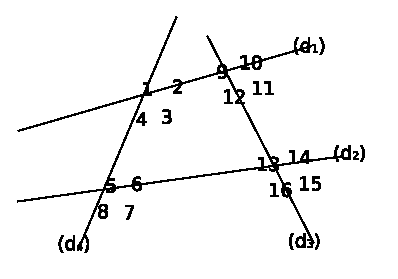
\includegraphics[width=.8\linewidth]{exoEnt14}
\end{center}

\end{exercice}



\begin{exercice}[Recherche de mesures d'angles]
\begin{enumerate}
\item Nomme deux paires d'angles de la figure :
    \begin{itemize}
    \item alternes-internes aigus ;
    \item alternes-internes de même mesure ;
    \item correspondants aigus ;
    \item supplémentaires et non adjacents.
    \end{itemize}
    
\begin{center}
    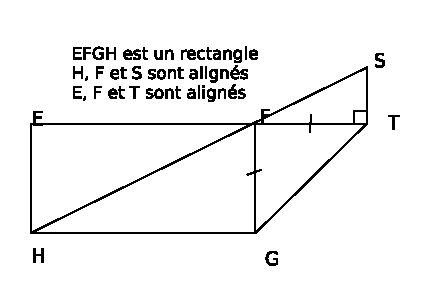
\includegraphics[width=.9\linewidth]{exoEnt15}
\end{center}

\item Sachant de plus que $\widehat{EFH}$ = 27°, calcule la mesure de l'angle $\widehat{SFT}$ puis celle de $\widehat{SFG}$.
\end{enumerate}
\end{exercice}

\columnbreak
\serie{Caractériser des droites parallèles par les angles}



\begin{exercice}
Dans chaque cas, dire si les droites $(d_1)$ et $(d_2)$ sont ou non parallèles et pourquoi.
\begin{center}
    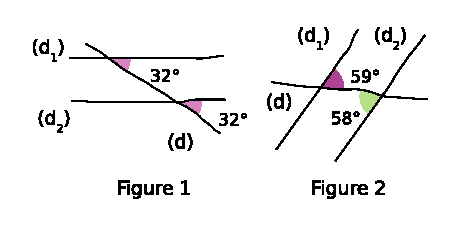
\includegraphics[width=.8\linewidth]{exoEnt16}
\end{center}
\end{exercice} 



\begin{exercice}[Le coup des équerres !]
Arnaud a placé ses deux équerres identiques sur la droite $(d)$ comme l'illustre le schéma ci-dessous.

\begin{center}
    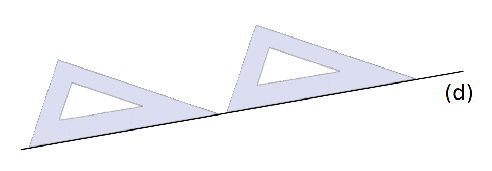
\includegraphics[width=.8\linewidth]{exoEnt17}
\end{center}

\begin{enumerate}
\item Il affirme que, de cette façon, il peut tracer des droites parallèles. Est-ce vrai et pourquoi ?
\item Quelles seraient les autres façons de positionner les équerres pour obtenir le même résultat ?
\end{enumerate}
\end{exercice} 



\begin{exercice}[Angles et droites parallèles]

\begin{center}
    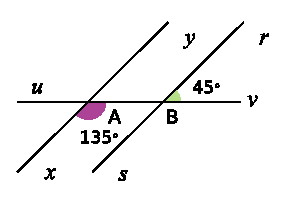
\includegraphics[width=.8\linewidth]{exoEnt18}
\end{center}

\begin{enumerate}
\item Calcule la mesure de l'angle $\widehat{uBr}$.
\item Les droites $(xy)$ et $(sr)$ sont-elles parallèles ? Justifie ta réponse.
\end{enumerate}
\end{exercice}



\columnbreak
\serie{Calculer des angles formés par des\\ droites parallèles}





\begin{exercice}[Parallèles ?]
Sur la figure ci-dessous, les angles $\widehat{BAE}$ et $\widehat{FEO}$ sont égaux à 58°.

\begin{center}
    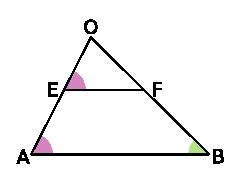
\includegraphics[width=.7\linewidth]{exoEnt19}
\end{center}

\begin{enumerate}
\item Que peux-tu dire des droites $(EF)$ et $(AB)$ ? Justifie ta réponse.
\item On sait de plus que la mesure de l'angle $\widehat{FBA}$ est 45°. Déduis-en la mesure de l'angle $\widehat{OFE}$. Justifie ta réponse.
\end{enumerate}
\end{exercice}


\begin{exercice}[Droites parallèles]

\begin{center}
    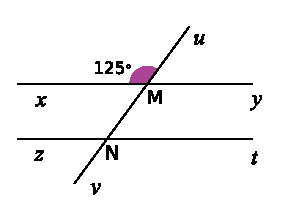
\includegraphics[width=.7\linewidth]{exoEnt20}
\end{center}

Sur la figure ci-dessus, les droites $(xy)$ et $(zt)$ sont parallèles. L'angle $\widehat{xMu}$ vaut 125°.
\begin{enumerate}
\item Donne la mesure de l'angle $\widehat{vMy}$. Justifie ta réponse.
\item Donne d'autres angles dont la mesure est de 125°. Justifie ta réponse.
\end{enumerate}
\end{exercice}

\newpage
\begin{exercice}[Angles supplémentaires]
                        
\begin{center}
    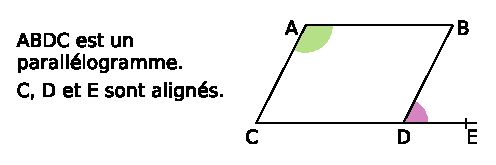
\includegraphics[width=\linewidth]{exoEnt21}
\end{center}
                                 
\begin{enumerate}
\item Justifie que les angles $\widehat{BAC}$ et $\widehat{BDC}$ sont de même mesure.
\item Que dire des angles $\widehat{BDC}$ et $\widehat{BDE}$ ? Pourquoi ? Justifie alors que les deux angles marqués sont supplémentaires.
\end{enumerate}
\end{exercice}

\columnbreak
\begin{exercice}[Zigzag]

\begin{center}
    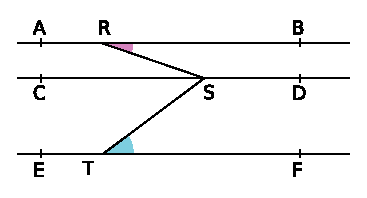
\includegraphics[width=.8\linewidth]{exoEnt22}
\end{center}

Sur la figure ci-dessus :
\begin{itemize}
    \item les droites $(AB)$, $(CD)$ et $(EF)$ sont parallèles ;
    \item $R$ est un point de la droite $(AB)$, $S$ est un point de la droite $(CD)$ et $T$ est un point de la droite $(EF)$ tels que : $\widehat{BRS}$ = 20° et $\widehat{RST}$ = 57°.
\end{itemize}

Calcule la mesure de l'angle $\widehat{STF}$.
\end{exercice}


\begin{exercice}
Construis à l'aide de \emph{TracenPoche} un quadrilatère $EFGH$ ayant deux angles droits, en $E$ et en $G$.
\begin{enumerate}
\item Affiche la mesure des angles $\widehat{EFG}$ et $\widehat{EHG}$. Que remarques-tu ?
\item Trace le segment $[FH]$. En raisonnant dans les triangles $EFH$ et $FHG$, démontre que $\widehat{EFG}$ et $\widehat{EHG}$ sont supplémentaires.
\end{enumerate}
\end{exercice}

\end{colonne*exercice}


\exercicesappr
\begin{colonne*exercice}
\begin{exercice}
Dans chaque cas, précise si les droites $(d_1)$ et $(d_2)$ sont ou non parallèles et pourquoi.

\begin{center}
    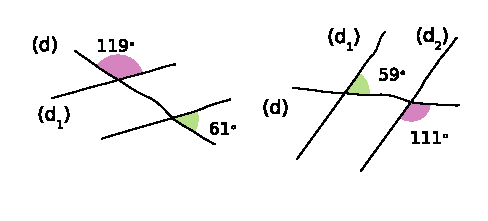
\includegraphics[width=\linewidth]{exoApp1}
\end{center}

\end{exercice}



\begin{exercice}[Triangle isocèle]

\begin{center}
    \includegraphics[width=.8\linewidth]{exoApp2}
\end{center}

La figure ci-dessus est telle que :
\begin{itemize}
    \item $B$, $A$ et $D$ sont des points alignés ;
    \item $\widehat{BAC}$ et $\widehat{ACD}$ sont supplémentaires ;
    \item $\widehat{BAC}$= 110°.
\end{itemize}

\begin{enumerate}
\item Montre, en justifiant, que les angles $\widehat{DAC}$ et $\widehat{ACD}$ sont égaux à 70°.
\item Montre alors que le triangle $ADC$ est isocèle.
\item De plus, l'angle $\widehat{ACB}$ mesure 50°. Montre, en justifiant, que les angles $\widehat{BCA}$ et $\widehat{ADC}$ sont complémentaires.
\item Trouve, en justifiant, deux autres paires d'angles complémentaires.
\end{enumerate}
\end{exercice}




\begin{exercice}[Parallèles ou non ?]

\begin{center}
    \includegraphics[width=.8\linewidth]{exoApp3}
\end{center}

La figure ci-dessus est tracée à main levée.

\begin{enumerate}
\item Calcule la mesure de l'angle $\widehat{LON}$.
\item Déduis-en la mesure de l'angle $\widehat{ONL}$.
\item Détermine alors si les droites $(LN)$ et $(MP)$ sont parallèles.
\item Sachant que les segments $[LN]$ et $[MP]$ sont de même longueur, détermine la nature du quadrilatère $LNPM$.
\end{enumerate}
\end{exercice}




\begin{exercice}[Un isocèle de plus]

\begin{center}
    \includegraphics[width=.6\linewidth]{exoApp4}
\end{center}

La figure ci-dessus est telle que :
\begin{itemize}
    \item les droites $(RO)$ et $(SN)$ sont sécantes en $T$ ;
    \item le triangle $RST$ est isocèle en $R$ ;
    \item les droites $(RS)$ et $(NO)$ sont parallèles.
\end{itemize}

Montre que le triangle $TNO$ est isocèle.
\end{exercice}




\begin{exercice}[Un périscope de fortune !]

\begin{enumerate}
\item Fais une recherche sur Internet concernant la loi de réflexion de la lumière.
\item Le schéma ci-dessous illustre un rayon de lumière qui se réfléchit sur un miroir avec un angle de 30°. Détermine $\hat{x}$ et $\hat{y}$. Justifie.

\begin{center}
    \includegraphics[width=.8\linewidth]{exoApp5}
\end{center}

\item Éric a construit un périscope avec une boîte de carton et deux miroirs parallèles comme l'illustre le schéma ci-dessous.

\begin{center}
    \includegraphics[width=.8\linewidth]{exoApp6}
\end{center}

\begin{itemize}
    \item Si un rayon entre horizontalement dans le périscope, en sortira-t-il horizontalement aussi ?
    
    (Tu pourras montrer que les rayons d'entrée et de sortie sont parallèles.)
    \item Ce résultat dépend-il de l'inclinaison des miroirs parallèles ?
    
    (Autrement dit, a-t-on le même résultat si l'angle formé par le rayon et le miroir est différent de 45° ?)
\end{itemize}
\end{enumerate}
\end{exercice}

\end{colonne*exercice}

\connaissances
\QCMautoevaluation{Pour chaque question, plusieurs réponses sont proposées. Déterminer celles qui sont correctes.}

\begin{QCM}

\begin{GroupeQCM}


\begin{exercice}
Parmi les couples d'angles suivants, quels sont ceux qui sont complémentaires ?
\begin{ChoixQCM}{2}
\item $\widehat{FEG}=8$° et $\widehat{HIK}=82$°
\item $\widehat{FEG}=90$° et $\widehat{HIK}=90$°
\item $\widehat{ABC}=73$° et $\widehat{STU}=107$°
\item $\widehat{FEG}=89,9$° et $\widehat{HIK}=0,1$°
\end{ChoixQCM}
\begin{corrige}
\reponseQCM{a}
\end{corrige}
\end{exercice}
\end{GroupeQCM}



\begin{EnonceCommunQCM}
Les questions \RefQCM{Aqcm1} et \RefQCM{Aqcm2} se rapportent à la figure ci-dessous.
\begin{center}
    \includegraphics[width=.25\linewidth]{qcm1}
    
    $E$, $R$ et $I$ sont alignés.
\end{center}
\end{EnonceCommunQCM}

\begin{GroupeQCM}


\begin{exercice}\label{Aqcm1}
Les angles...
\begin{ChoixQCM}{2}
\item $\widehat{ERH}$ et $\widehat{HRI}$ sont supplémentaires
\item $\widehat{FRG}$ et $\widehat{HRI}$ sont adjacents
\item $\widehat{ERG}$ et $\widehat{FRI}$ sont supplémentaires
\item $\widehat{FRG}$ et $\widehat{GRH}$ sont adjacents
\end{ChoixQCM}
\begin{corrige}
\reponseQCM{a}
\end{corrige}
\end{exercice}





\begin{exercice}\label{Aqcm2}
L'angle...
\begin{ChoixQCM}{2}
\item $\widehat{FRG}$ est le complémentaire de $\widehat{GRH}$
\item $\widehat{FRE}$ est le complémentaire de $\widehat{HRI}$
\item $\widehat{ERF}$ est le complémentaire de $\widehat{FRI}$
\item $\widehat{GRH}$ est le complémentaire de $\widehat{HRI}$
\end{ChoixQCM}
\begin{corrige}
\reponseQCM{a}
\end{corrige}
\end{exercice}
\end{GroupeQCM}
\end{QCM}

\begin{QCM}

\begin{EnonceCommunQCM}
Les questions \RefQCM{Aqcm3}, \RefQCM{Aqcm4} et \RefQCM{Aqcm5} se rapportent à la figure ci-dessous.
\begin{center}
    \includegraphics[width=.25\linewidth]{qcm2}
    
    $(AD)$ et $(FH)$ sont parallèles.
\end{center}
\end{EnonceCommunQCM}

\begin{GroupeQCM}

\begin{exercice}\label{Aqcm3}

\begin{ChoixQCM}{2}
\item $\widehat{ACH}$ et $\widehat{BCD}$ sont opposés par le sommet
\item $\widehat{CDF}$ et $\widehat{BCD}$ sont opposés par le sommet
\item $\widehat{ACH}$ et $\widehat{BCD}$ sont adjacents
\item $\widehat{BCD}$ et $\widehat{CHF}$ sont correspondants
\end{ChoixQCM}
\begin{corrige}
\reponseQCM{a}
\end{corrige}
\end{exercice}




\begin{exercice}\label{Aqcm4}

\begin{ChoixQCM}{4}
\item $\widehat{BCD}=100$°
\item $\widehat{BHF}=100$°
\item $\widehat{BCA}=100$°
\item $\widehat{DCH}=100$°
\end{ChoixQCM}
\begin{corrige}
\reponseQCM{a}
\end{corrige}
\end{exercice}




\begin{exercice}\label{Aqcm5}

\begin{ChoixQCM}{4}
\item $\widehat{CDF}=40$°
\item $\widehat{BFH}=50$°
\item $\widehat{DCH}=80$°
\item $\widehat{CDF}=100$°
\end{ChoixQCM}
\begin{corrige}
\reponseQCM{a}
\end{corrige}
\end{exercice}

\end{GroupeQCM}
\end{QCM}



\begin{QCM}

\begin{GroupeQCM}

\begin{exercice}
\begin{center}
    \includegraphics[width=.25\linewidth]{qcm3}
\end{center}
\begin{ChoixQCM}{4}
\item Si les angles roses sont égaux alors $(d)$ et $(d')$ sont parallèles
\item Si $(d)$ et $(d')$ sont parallèles alors les angles roses sont égaux
\item Les angles roses sont correspondants
\item Les angles roses sont alternes-internes
\end{ChoixQCM}
\begin{corrige}
\reponseQCM{a}
\end{corrige}
\end{exercice}



\begin{exercice}
Quelles sont les affirmations vraies ?
\begin{ChoixQCM}{4}
\item $\widehat{OUG}$ et $\widehat{ZKL}$ sont opposés par le sommet
\item Deux angles alternes-internes peuvent être opposés par le sommet
\item Deux angles correspondants peuvent être opposés par le sommet
\item Le supplémentaire d'un angle aigu est obtus
\end{ChoixQCM}
\begin{corrige}
\reponseQCM{a}
\end{corrige}
\end{exercice}




\begin{exercice}
\begin{center}
    \includegraphics[width=.25\linewidth]{qcm4}
    
    $(TR)$ et $(SU)$ sont parallèles et $\widehat{REA}$=60°.
\end{center}
\begin{ChoixQCM}{4}
\item $\widehat{EAS}=60$°
\item $\widehat{TEA}=120$°
\item $\widehat{EAU}=60$°
\item $\widehat{EAU}=90$°
\end{ChoixQCM}
\begin{corrige}
\reponseQCM{a}
\end{corrige}
\end{exercice}

\end{GroupeQCM}
\end{QCM}

\TravauxPratiques
\begin{TP}[Triominos avec les angles]


\textbf{1\up{ère} étape : calculer et justifier}

\begin{enumerate}
\item Voici six figures. Pour chacune d'elles, calculez, en justifiant votre calcul, l'angle marqué par un point d'interrogation. (Les droites d'une même couleur sont parallèles.)

\begin{center}
    \includegraphics[width=.6\linewidth]{tabImage}
\end{center}


\item Voici six énoncés. Pour chacun d'eux, répondez à la question en justifiant la réponse :

\begin{center}
    \includegraphics[width=.6\linewidth]{tabType}
\end{center}


\vspace{1em}\textbf{2\up{e} étape : construction des triominos}\vspace{1em}

\item \label{AtpTabType} Voici un tableau qui va vous permettre de construire le jeu de triominos. 

\begin{center}
    \includegraphics[width=.6\linewidth]{tableau}
\end{center}

Toutes les cases d'une même colonne renvoient à l'angle indiqué en ligne 1. Par exemple, les cases F2, F3... renvoient à un angle de 110°.

Pour le type \textbf{t3}, mettez aussi des exemples d'angles correspondants.

\item Dans une feuille blanche au format A4, construisez 10 triangles équilatéraux de 9 cm de côté. Utilisez une seconde feuille pour obtenir 20 triominos au total. Complétez chacun d'eux avec les énoncés ou constructions indiqués dans le tableau de la question \ref{AtpTabType}. en respectant l'ordre donné ci-dessous. Pour vous aider, voici un exemple pour le premier triomino de la série :

\hfill\includegraphics[width=.15\linewidth]{tp7} \hfill \includegraphics[width=.3\linewidth]{tp8}\hfill\phantom{.}
 
\begin{center}
    \includegraphics[width=.75\linewidth]{tp9}
    
    \includegraphics[width=.75\linewidth]{tp10}
\end{center}

\vspace{1em}\textbf{3\up{e} étape : par équipe de deux joueurs}\vspace{1em}

Retournez tous les triominos pour former la pioche. Chaque joueur en prend quatre.      

Un triomino est tiré dans la pioche pour servir de départ. Chaque joueur place à son tour un triomino. (Les côtés qui se touchent doivent correspondre à des angles égaux.)

Si le joueur ne peut pas jouer, il passe son tour \textbf{et} pioche. Le premier joueur qui n'a plus de triomino est déclaré vainqueur.

\textbf{Attention} : si un joueur se trompe en plaçant un triomino, il doit le reprendre et tirer un triomino supplémentaire dans la pioche ; c'est alors à son adversaire de jouer...
\end{enumerate}

\end{TP}

\recreation % avec R majuscule pour saut de page
\begin{enigme}[Un problème de construction]
Trace une droite $(d)$ et place un point $A$ n'appartenant pas à $(d)$.

Construis un triangle équilatéral dont un des sommets est $A$ et les deux autres sommets sont deux points de la droite $(d)$.

Propose une méthode de construction à l'aide d'un logiciel de géométrie dynamique.
\end{enigme}


